% will smith citation 

\documentclass[10pt,letterpaper]{article}
\usepackage{graphicx}
\usepackage{cogsci}
\usepackage{pslatex}
\usepackage{apacite2}
\usepackage{subfigure}
\usepackage{amsmath}
\usepackage{amssymb}
\usepackage{tikz}
\usepackage{marvosym}
\usepackage{wasysym}
\usepackage{times}
\usepackage{epsfig}
\usepackage{tabularx}
\usepackage[titletoc,toc,title]{appendix}


\usetikzlibrary{decorations.pathreplacing,calc}
\title{Discovering new Signatures of Joint Attention in Egocentric Video}

\author{{\bf Guido Pusiol}\\ 
\texttt{guido@cs.stanford.edu} \\
Department of Computer Science\\
Department of Psychology \\
Stanford University
  \And {\bf Laura Soriano} \\ 
\texttt{lsoriano@stanford.edu} \\
Department of Psychology\\
Stanford University 
\And {\bf Li Fei-Fei} \\
\texttt{feifeili@stanford.edu} \\
  Department of Computer Science\\
Stanford University 
\And {\bf Michael C. Frank} \\ 
\texttt{mcfrank@stanford.edu} \\
  Department of Psychology\\
Stanford University}
  
\newcommand{\argmax}[1]{\underset{#1}{\operatorname{arg}\,\operatorname{max}}\;}
\begin{document}
\maketitle

\begin{abstract}

\textbf{Keywords:} 
Joint attention; computer vision; child development; social cognition. 
\end{abstract}



\section{Introduction}

How do young children begin learning the meanings of words? Across cultures, early vocabulary includes names for people, simple social routines, animals, and objects \cite{tardif2008}, suggesting that the earliest words are learned through interaction and play with others \cite{bruner1985}.  Identifying a caregiver's intended referent is a critical part of learning meaning within these interactions, and this identification is often accomplished through \emph{joint attention}.

Joint attention describes periods of time when both child and caregiver are attending to the same thing and when both know that the other is attending to it \cite<for the remainder of the paper we will talk informally about joint attention---JA---as both the phenomenon and the period of time during which it happens;>{carpenter2011}.  A typical example of JA is a situation where an adult and child are playing with a toy and the infant alternates gaze between the adult and the toy \cite{carpenter1998}. 

The capacity for JA gradually develops over the first two years of life and usually begins to emerge between 9 and 12 months of age \cite{morales2000}, coinciding with the beginnings of language learning. In addition, the skills that enable JA (e.g. pointing, following a caregiver's gaze to a distal target) and the amount of time that children spend in JA with their caregivers are both strong predictors of children's early vocabulary growth \cite{carpenter1998,brooks2008,tomasello1983}. 

How do children know that they are in joint attention with a caregiver? From an external perspective, joint attention has typically been defined by a sequence of events: (1) one member of the interaction (child or caregiver) directs the other member’s attention to an object, (2) both members focus visually on the object, and (3) the child indicates awareness of the caregiver  \cite{tomasello1986}. 

Previous work has typically used children's gaze as the main indicator of JA, but, from the perspective of both the child and the data analyst, this method has several issues. First, gaze is neither necessary nor sufficient for JA. It is possible to attend jointly through the hands---as with a child reading a picturebook on a parent's lap---or for the child to follow gaze to a distal target and then signal awareness by moving towards it or reaching for it. Indeed, eye-tracking studies investigating signals to reference find that manual signals are far more effective than gaze in manipulating young children's attention \cite{yurovsky2013}. Second, young children may not have perceptual access to their caregiver's gaze most of the time. Recent studies using head-mounted cameras and eye-trackers suggest that children are more often looking at the objects in front of them than at the faces of their caregivers \cite{smith2011,franchak2011,frank2013}. Third, parents most often look at their children, not at the object they are talking about \cite{frank2013b}. Thus, gaze alone is at best a noisy cue for the identification of JA, either for the child or for the researcher attempting to identify JA in a large dataset.

The goal of our current work is to discover other signals of joint attention. There are two purposes to this investigation. The first is data analytic: A better understanding of how to extract JA episodes from video could be a powerful tool for analyzing video corpora. The second is psychological: The unsupervised extraction of JA episodes from video could give hints regarding robust cues that children might use in addition to, or even in lieu of, gaze. 

We use two data sources to gain information about the social interaction between child and caregiver: head-mounted and fixed camera videos. Our approach is unsupervised discovery. We first use computational methods to extract a number of different features---including episodes of static attention, faces, and objects that are currently in motion. We then  examine the correlations between these features (and higher-level clusters of these features) and hand-coded joint attentional episodes. Our results suggest that there are a number of redundant perceptual cues to JA, and that some of these may be more robust and readily accessible to children than gaze. 



\begin{figure}[h]
     \begin{center}
        \subfigure[todo]{%
           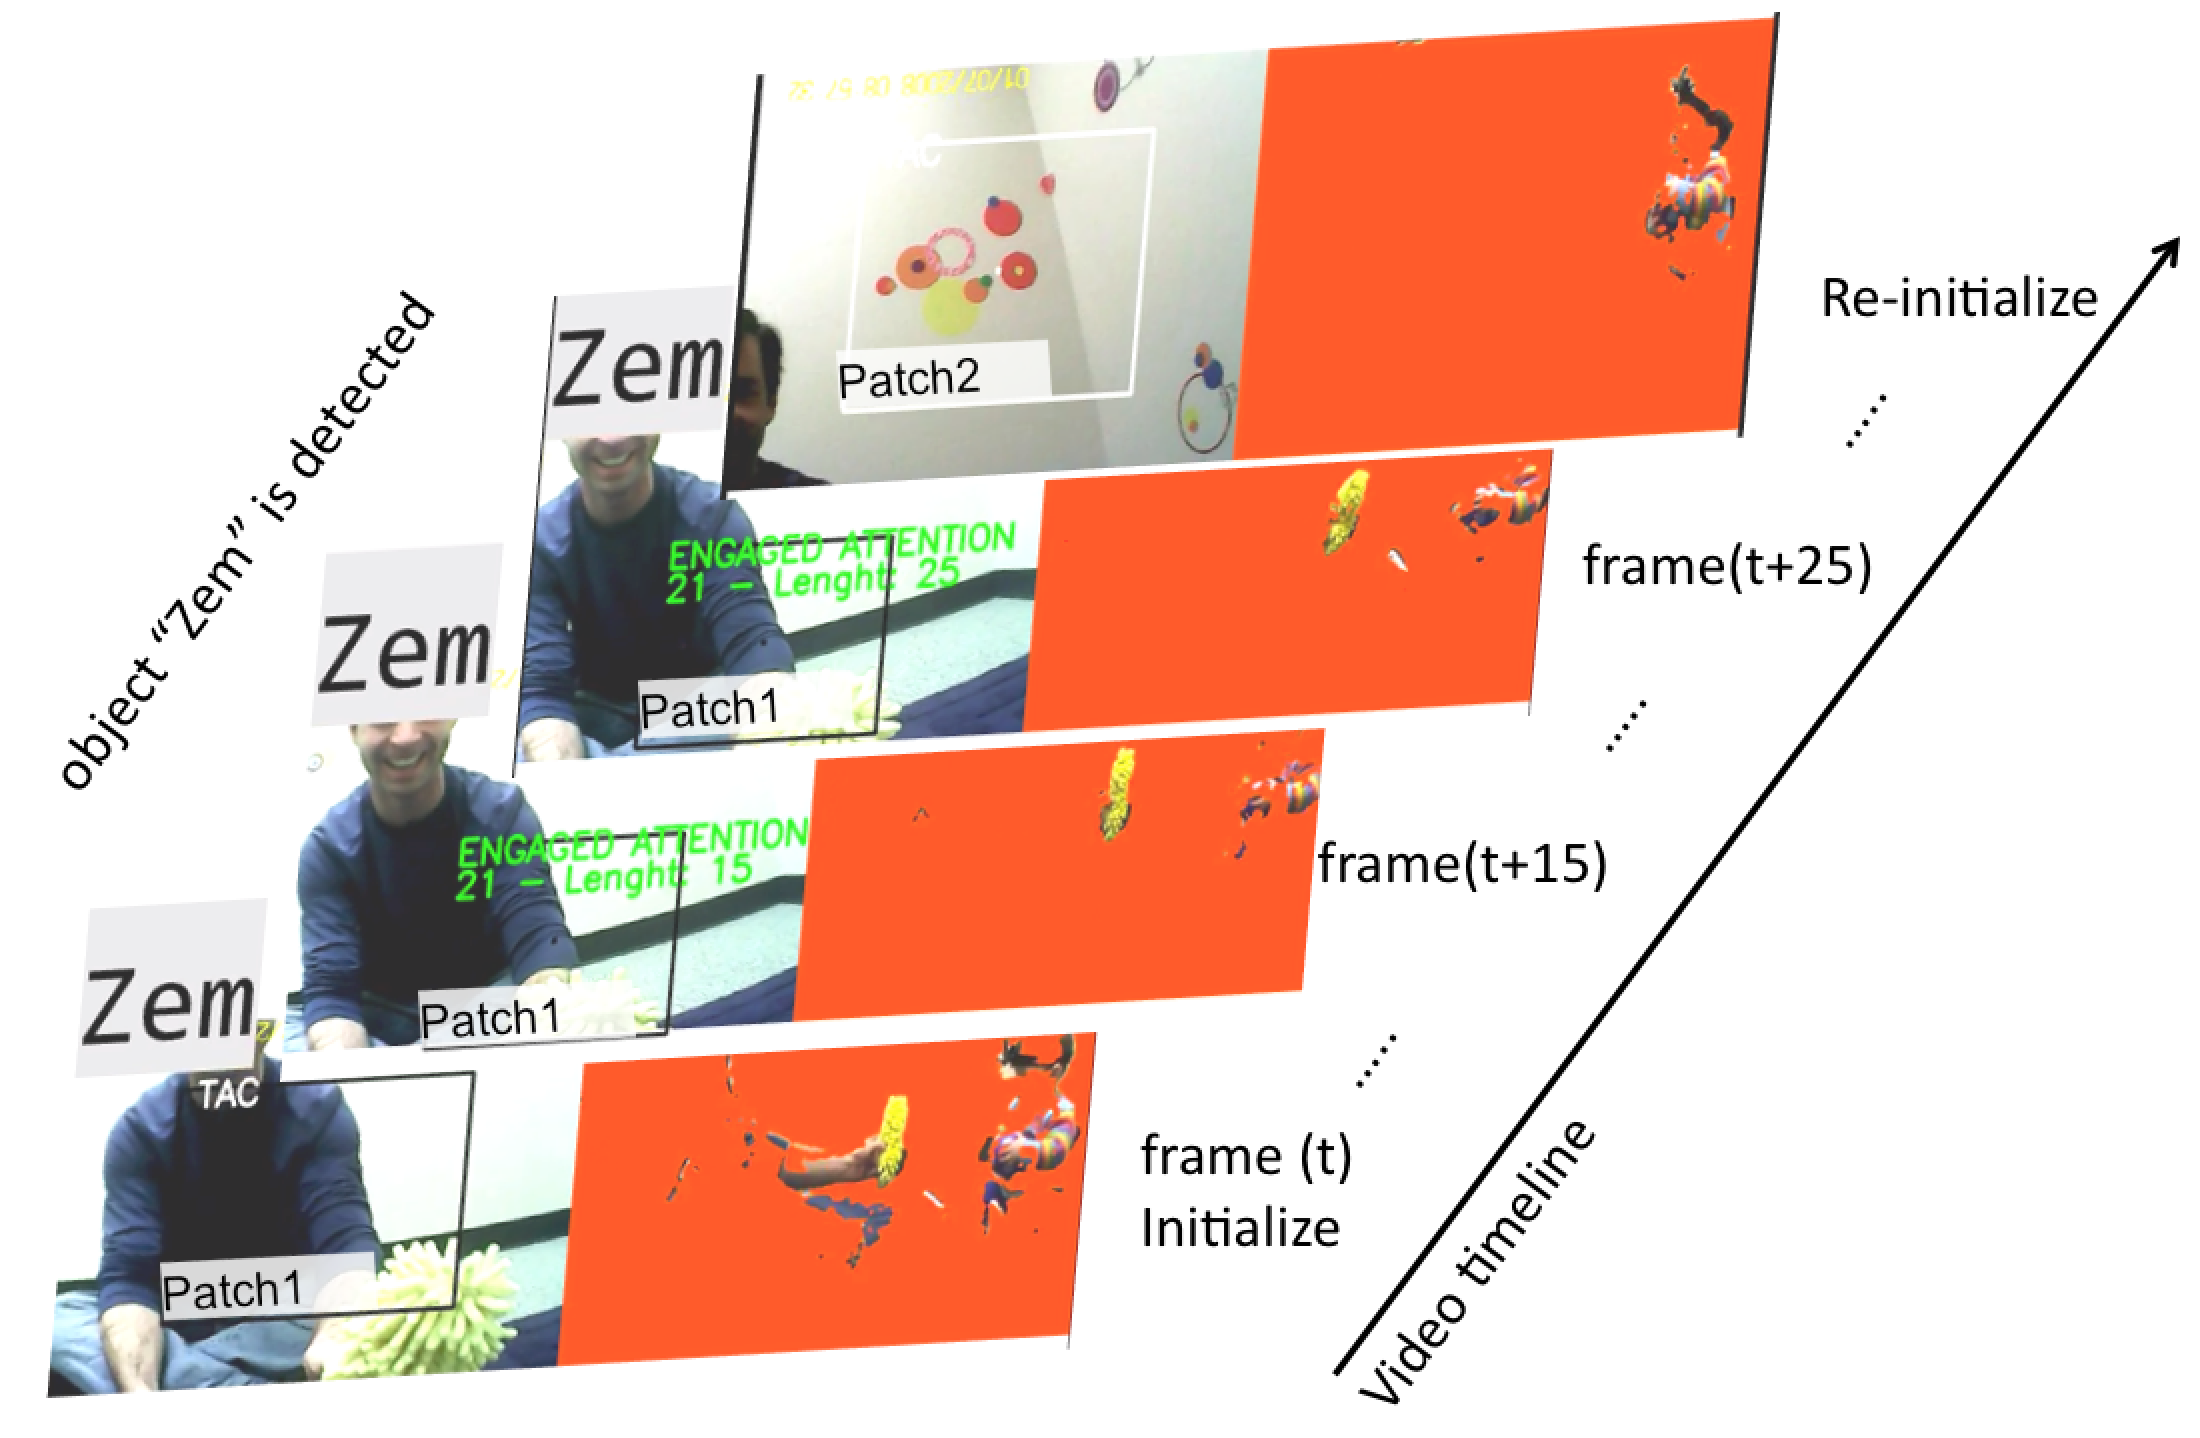
\includegraphics[width=1\linewidth]{Image/cogsci} 
           }
          \end{center}
    \caption{todo... 
     }
   \label{fig:main}
\end{figure}

\section{Features Computation}
%%%%%% FIGURE FACE DETECTION
{\bf 1. Face Detection.} Traditional off-the-shelf face detection algorithms fall short to detect the parent faces in the baby-cam dataset. Face detectors work accurately when the test dataset present low variability on the testing dataset and the distance is above 1 meter (e.g. Facebook like pictures). In the baby perspective other type of face configurations appear. Faces appear partially, blurred and with big size and texture variability (fig. \ref{fig:faces}) making their detection challenging. We address the problem by with a semi automated adaptive algorithm \cite{kalal}. The algorithm requires manual user input (selecting a face example per video) for its initialization, but then needed no additional human intervention. The algorithm uses new pixel patches in the trajectory of an optical-flow based tracker to train and update a face detector. The optical flow tracker and the face detector work in parallel. If the face detector finds a location in a new frame exhibiting a high similarity to its stored template, the tracker is re-initialised on that location. Otherwise, the tracker uses the optical flow to decide the location of a face in the new frame. The primary advantage of the algorithm is the use of motion for face detection: Following the movement of the pixels that define a face it is possible for the algorithm to adapt to new morphologies (i.e. different face poses).
\begin{figure}[h]
          \subfigure[Blurred]{
             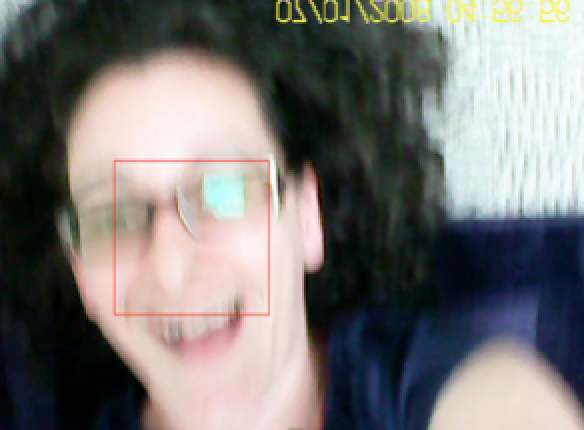
\includegraphics[width=1in,height= 1in]{Image/a}
             }    
            \subfigure[Partial face]{
            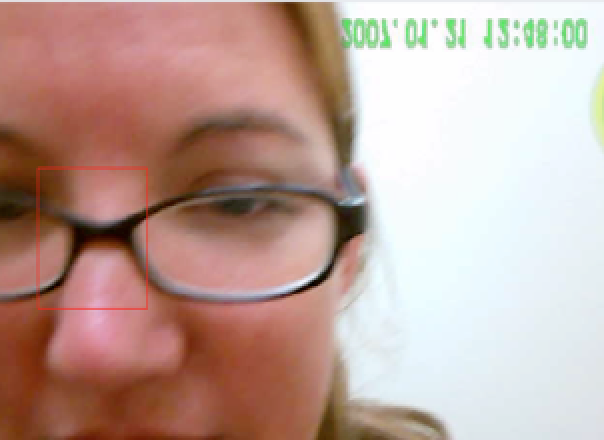
\includegraphics[width=1in,height= 1in]{Image/c} 
            }
             \subfigure[Low texture]{          
             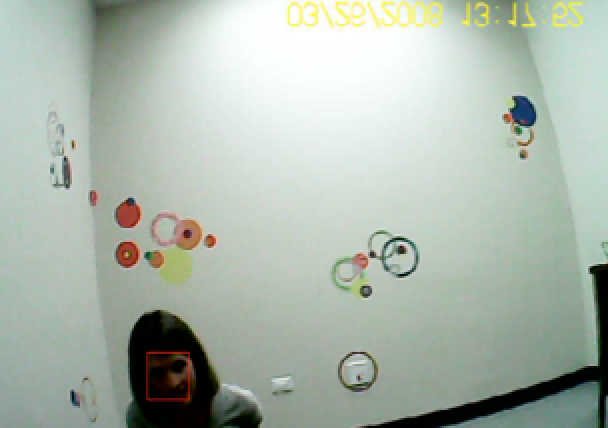
\includegraphics[width=1in,height= 1in]{Image/d} 
             }
    
    \caption{Results (red rectangles) of our face detector in difficult frames.
 }
\label{fig:faces}
\end{figure}
{\bf Precision.} We evaluate the face detector using 37 videos of children's head mounted cameras.  Our evaluation compares the automatically detected faces with human ground truth annotations. The metrics:  precision = .92; recall = .99; true Negatives = 93; accuracy = 96 outperform the state of the art \cite{dpmface} due to the active-learning stage of the algorithm.\\

{\bf 2. Handled object detection and tracking.} We aim at exploring cues of joint attention expressed by hand interactions. The detection of objects being moved even when they are not fully in the visual scope of the children could indicate that the joint attention is established. To automatically track moving objects we first compute the foreground mask representing the moving parts of the video. Understanding the moving parts helps to filter out static patches which can confuse the tracker -figure  \ref{fig:subfigures} (a)-, and also to filter out non manipulated objects of interest - figure \ref{fig:subfigures} (b)-\\

%For that we make extensive use of local binary patterns as texture descriptors.
\begin{figure}[ht]
     \begin{center}
          \subfigure[Object of interest (i.e. yellow square) could be confused with other similar textures and color objects in the scene (i.e red squares). The background mask (bottom-right) is filtering the problems out.]{
        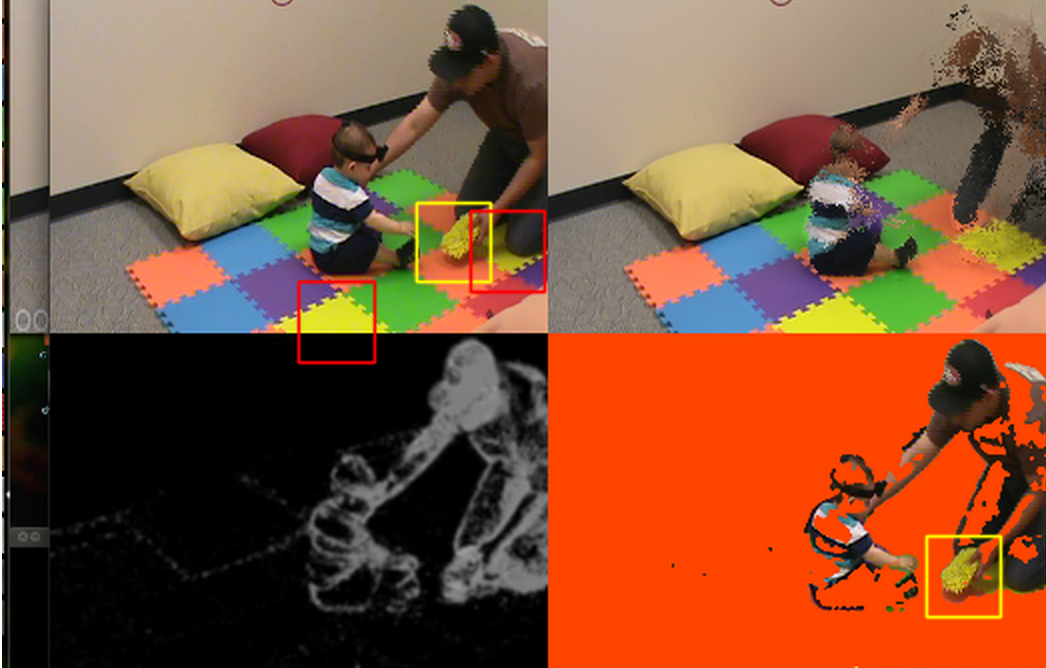
\includegraphics[width=0.8\linewidth]{Image/Zem}}
        \subfigure[Objects of interest are being handled and therefore are moving (i.e. yellow square). Forgotten objects (i.e red squares) are filtered out by the foreground mask.]{
        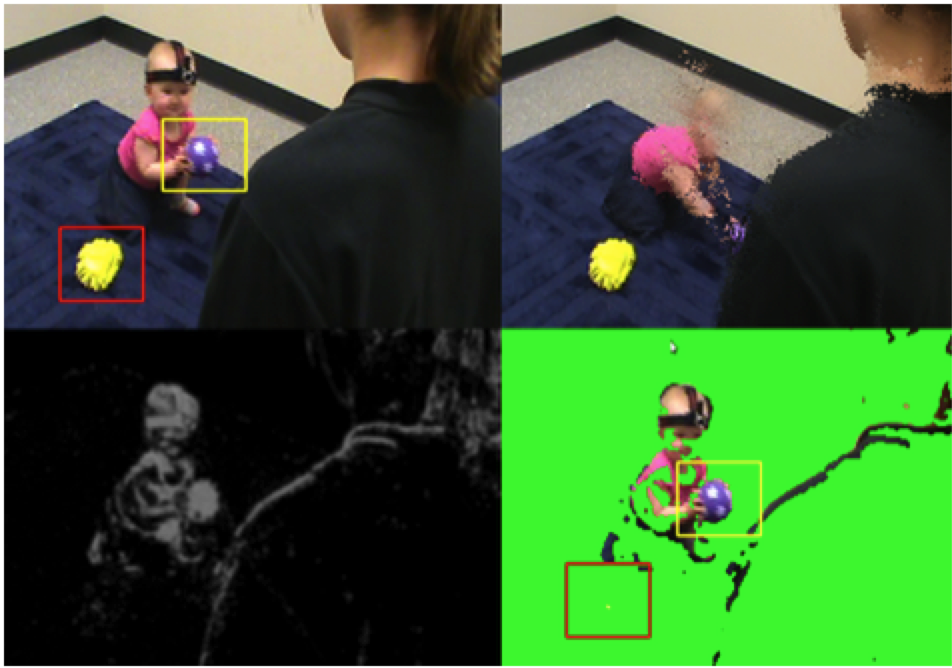
\includegraphics[width=0.8\linewidth]{Image/four}}
        \end{center}

    \caption{Foreground computation. In each image, top-left: original color frame, top-right: background model color vector ($I$), bottom-left: foreground weights, bottom-right: foreground extraction (i.e. orange or green pixels correspond to the background mask). (a) depicts the problem of similar texture and color of the scene and the object of interest. (b) represents the problem of uninteresting objects visible in the scene. Both problems are addressed at once with background/foreground segmentation filtering.}
   \label{fig:subfigures}
\end{figure}

{\bf 2.1. Foreground Modeling.} The goal is to construct and maintain a statistical representation of the scene to be modeled. Here, we chose to utilize both texture information and color information when modeling the background. The approach \cite{odobez1} exploits the Local Binary Pattern (LBP) feature as a measure of texture because of its good properties \cite{Halika}, along with an illumination invariant photometric distance measure in the RGB space.\\
The background model ${{B}^{t}(x)}$ of the pixel $x$ at the time $t$ is represented by a list of modes $\{ {m}^{t}_{k}(x)\}_{k=1\dots K}$. The modes register historic information of 7 features of the pixels color and surrounding texture. ${m}^{t}_{k} = \{I ,\hat{I},\breve{I}, {LBP}_{k}, w,  \hat{w}, P \}$. Where ${I}$ represents the average $RGB$ image vector. $\hat{I}$ and $\breve{I}$ are the maximal and minimal $RGB$ image vectors. {LBP} is the vector of local binary patterns computed at this mode.\\
The background model can learn up to $K^{max}$ different modes. For each new $I^{t}$ and $LBP^{t}$ a new mode is computed $m^{t-1}_{k}$ and the algorithm seeks to which learned mode $m^{t-1}_{k}$ the new mode maps to. The mapping is achieved by thresholding a distance (i.e $\tilde{k} = \underset{{k}}{\arg\min} ~ D(m^{t-1}_{k},m^{t}_{k})$). 1) If the new mode cannot be mapped to any of the learned ones and there is still space in the buffer ($K $\textless$ K^{max}$), then a new mode is initialized. 2) If there is a matched mode $m^{t-1}_{\tilde{k}}$, its representation is updated as follows:
\begin{equation}
   \begin{cases} 
     \breve{I}_{\tilde{k}}^{t} = min (I^{t}, (1 + \beta) \breve{I}_{\tilde{k}}^{t-1}), \\
     \hat{I}_{\tilde{k}}^{t} = max (I^{t}, (1 - \beta) \hat{I}_{\tilde{k}}^{t-1}), \\
     {I}_{\tilde{k}}^{t} = (1 + \alpha) {I}_{\tilde{k}}^{t-1} + \alpha	{I}^{t}, \\
     {LBP}_{\tilde{k}}^{t} = (1 + \alpha) {LBP}_{\tilde{k}}^{t-1} + \alpha	{LBP}^{t}, \\
     (*)w^{t}_{\tilde k}= (1 - \alpha^{i}_{w}) {w}_{\tilde{k}}^{t-1} + \alpha^{i}_{w},\\ ~~~ ~~~ ~~~ \alpha^{i}_{w}=\alpha_{w}(1+\tau\hat{w}^{t-1}_{k}) \\
     \hat{w}^{t}_{\tilde{k}} = max (\hat{w}^{t-1}_{\tilde{k}}, w^{t}_{\tilde{k}})\\
     L^{t}_{\tilde{k}} = 1+ max \{L^{t-1}_{k}\}_{k=1,\dots,K, k \neq \tilde{k}},\\ ~~~ ~~~ ~~~ if~~ L^{t}_{\tilde{k}}~=~0~and~T_{bw} $\textless$\hat{w}_{\tilde{k}}^{t} \\
   \end{cases} 
\end{equation}

where $\beta \in [0,1)$ is the learning rate of the min and max color vectors and $\alpha \in [0,1)$ is the learning rate of the color and texture information. The non matching modes of the previous model are assigned to the new model (i.e. $m^{t}{k}:=m^{t-1}{k}$ ) but their weights are decreased according to (*).
\\
After the update step, all nodes are sorted decreasingly according to their weight. And the background modes are the first $B^{t}$ modes that satisfy:
\begin {equation}\sum_{k=1}^{B^{t}} w_{k}^{t} / \sum_{k=1}^{K^{t}} w_{k}^{t} < TB \end{equation} where $TB  \in [0,1]$ is the background threshold.
Note that the use of both color and texture, the chances that moving foreground objects generate a consistent mode overtime (and beneÞciate from this effect) are quite small.\\

{\bf 2.2 Object tracking}. We are interested in detecting a tracking a set of objects (i.e. toys) components of triad when the parents and children are engaged in a JA episode. In particular the toys are being manipulated. The detection and tracking objects is performed over the foreground image. From a computer vision perspective, the objects are highly deformable making them hard to detect and track. The deformations are due to the changes of positions and hand-object occlusions that the object can take while is being manipulated. We have tried different appearance-based \cite{TLD} object detectors, and all of them failed. We have finally adopted to detect and track them by its color and relative size. We modified the cam-shift algorithm \cite{bradsky}, which is a specialization of  the well known mean-shift algorithm \cite{Meer2002}. The mean shift algorithm is a non-parametric technique that climbs the gradient of a probability distribution to find the nearest dominant mode (peak). In our case the distribution is based in color values. The algorithm initializes selecting a region containing the object of interest, and building a color histogram over the region. In a new frame, the algorithm will match the region size and the peaks of the color distribution using mean-shift and the euclidean distance. The figure \ref{fig:track} depicts examples of the detection and tracking of two different objects.\\
\begin{figure}[h!]
     \begin{center}
        \subfigure[Green object is detected]{
           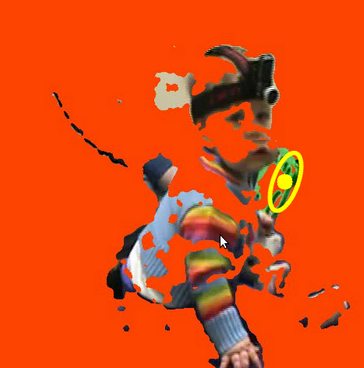
\includegraphics[width=0.4\linewidth]{Image/g2}
           \label{fig:tracking} 
           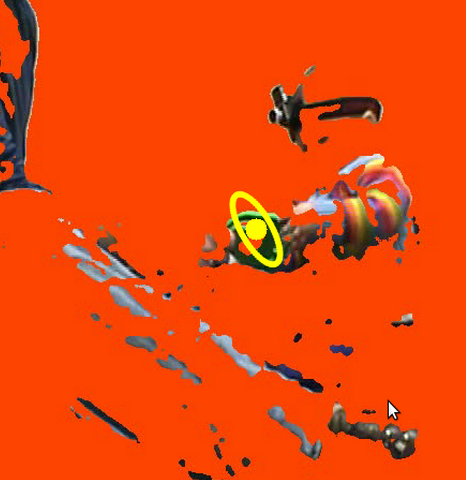
\includegraphics[width=0.4\linewidth]{Image/g4}
            }
          \subfigure[Zem is detected]{
           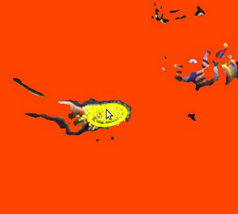
\includegraphics[width=0.45\linewidth]{Image/z1}

          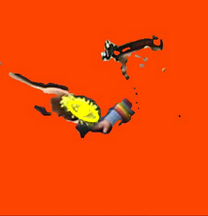
\includegraphics[width=0.4\linewidth]{Image/z2}
           \label{fig:tracking} }
         
    \end{center}
    \caption{(a) the green object is detected, its size and momentum is depicted by the yellow ellipse. (b)}
   \label{fig:track}
\end{figure}

%%%%%% ATTENTION MOTION  ATTENTION CHUNKS
{\bf 3. Attention Chunks:} 
The attention chunks capture the segments of video of a child engaged visually to a concept. They are extracted of the head camera
. The concept can be a concrete object (face, toy, etc.) or an abstract texture captured by the camera when the child's gaze is attending to an off-scope object (e.g. the child is handling a toy near his chest). The ideal case is to have eye trackers to understand the gaze of the baby, but such a configuration is very hard to achieve in uncontrolled environments. Thus, we use the head-cam information as a gaze estimator. Our approach is backed by psychophysical experiments that indicate eye gaze and head pose are coupled in various tasks \cite{Land1,Pelz}. The attention chunk is computed automatically. The algorithm is initializes by modeling a pixel-texture patch ($P_{i}$). 
For each new frame the algorithm will seek for a similar patch to the one observed in the previous frame. If the patch is matched, a new point is added to the patch trajectory. If the matching is not achieved, a new patch ($P_{i+1}$) is learned and the tracking algorithm is re-initialized. The base algorithm used for tracking is a version of a tracker by detection algorithm \cite{kalal}. An Attention Chunk is the video segment defined by the $start_{P}$ and $end_{P}$ frames of the tacked patch trajectory.
The figure \ref{fig:chunk} describes the basics of an attention chunk computation.\\
\begin{figure}[h]
\begin{center}
        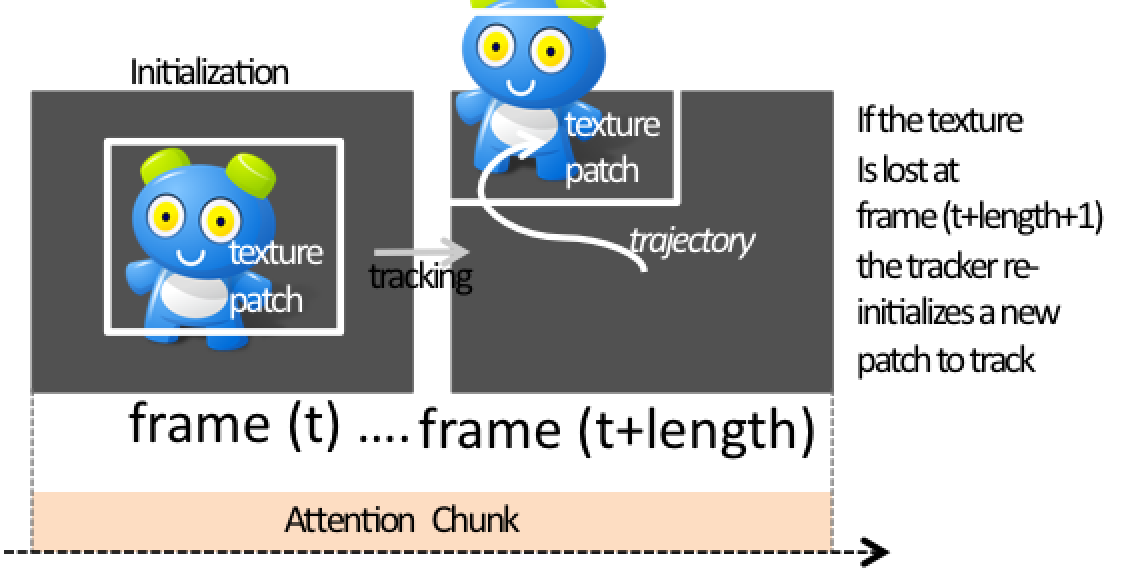
\includegraphics[width=0.5\linewidth]{Image/Attchunk}      
          \end{center}
    \caption{Attention chunk computation.}
   \label{fig:chunk}
\end{figure}
We perform analytics over the obtained chunk lengths to understand behavioral structures hidden in the data. We have categorized the extracted chunks by their duration in groups of children of different ages. We used 37 children head can videos (~20 min. each) grouped by age: 6, 12 and 16 month old. The average duration of the chunks is depicted in the figure \ref{fig:duration}. Younger children show to have longer episodes of attending to a spot. While the reasons will require of further discussion, our thoughts are that 16 month old children can walk and are more autonomous, and can avoid the parents imposition of attending to certain objects. The figure \ref{fig:buckets} depicts the temporal duration of the chunks distributed in buckets of 10ms in a log scale. The graph shows that the decay is proportionally symmetric among the different groups, most of the attention chunks are of short duration and there are not "distractors" (i.e. a TV) that interfere with our guided attention towards new objects. 

\begin{figure}[h]
\begin{center}
        \subfigure[Duration of attentional chunks ordered by children age 8,12 and 16 month old.]{%           
           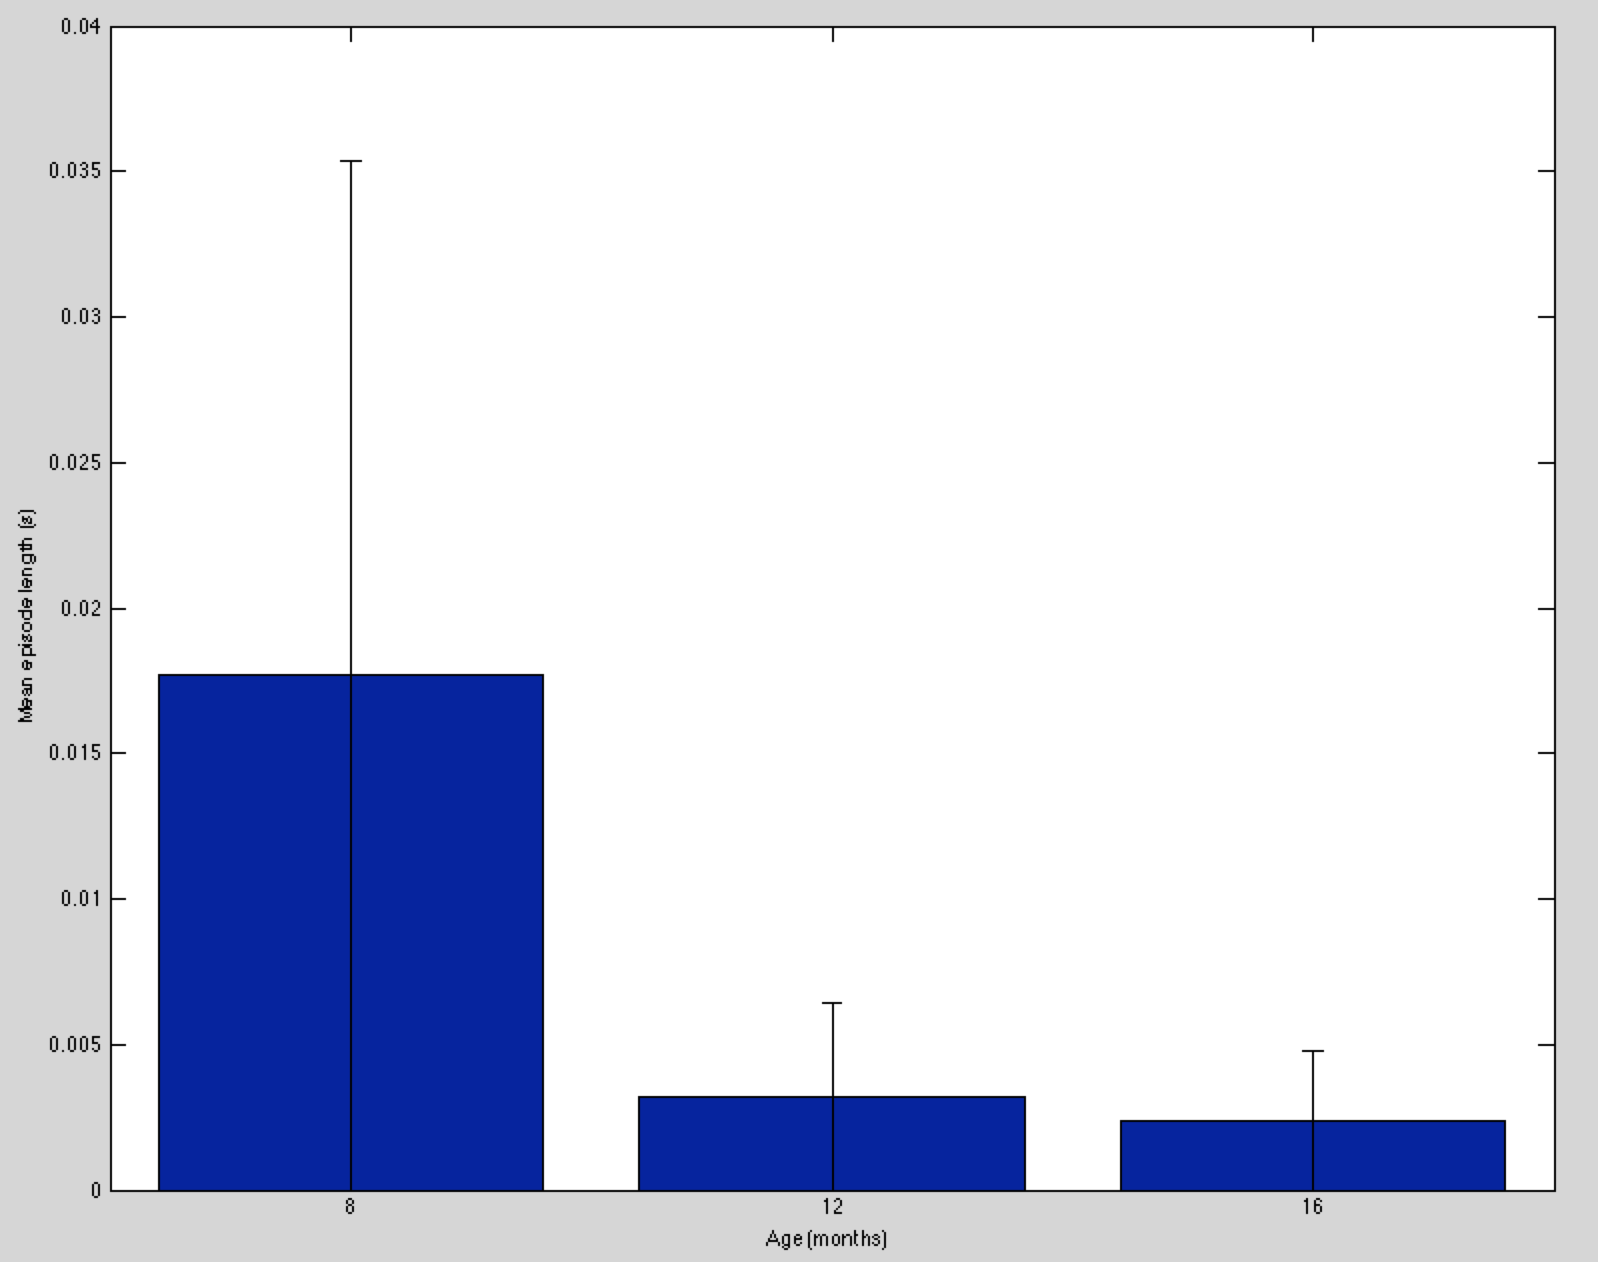
\includegraphics[width=0.5 \linewidth]{Image/log3}
           \label{fig:duration}
           }
           \subfigure[Duration of the attentional chunks distributed in buckets of 10ms and displayed in log scale (i.e. longer chunks appear to the right).]{%
           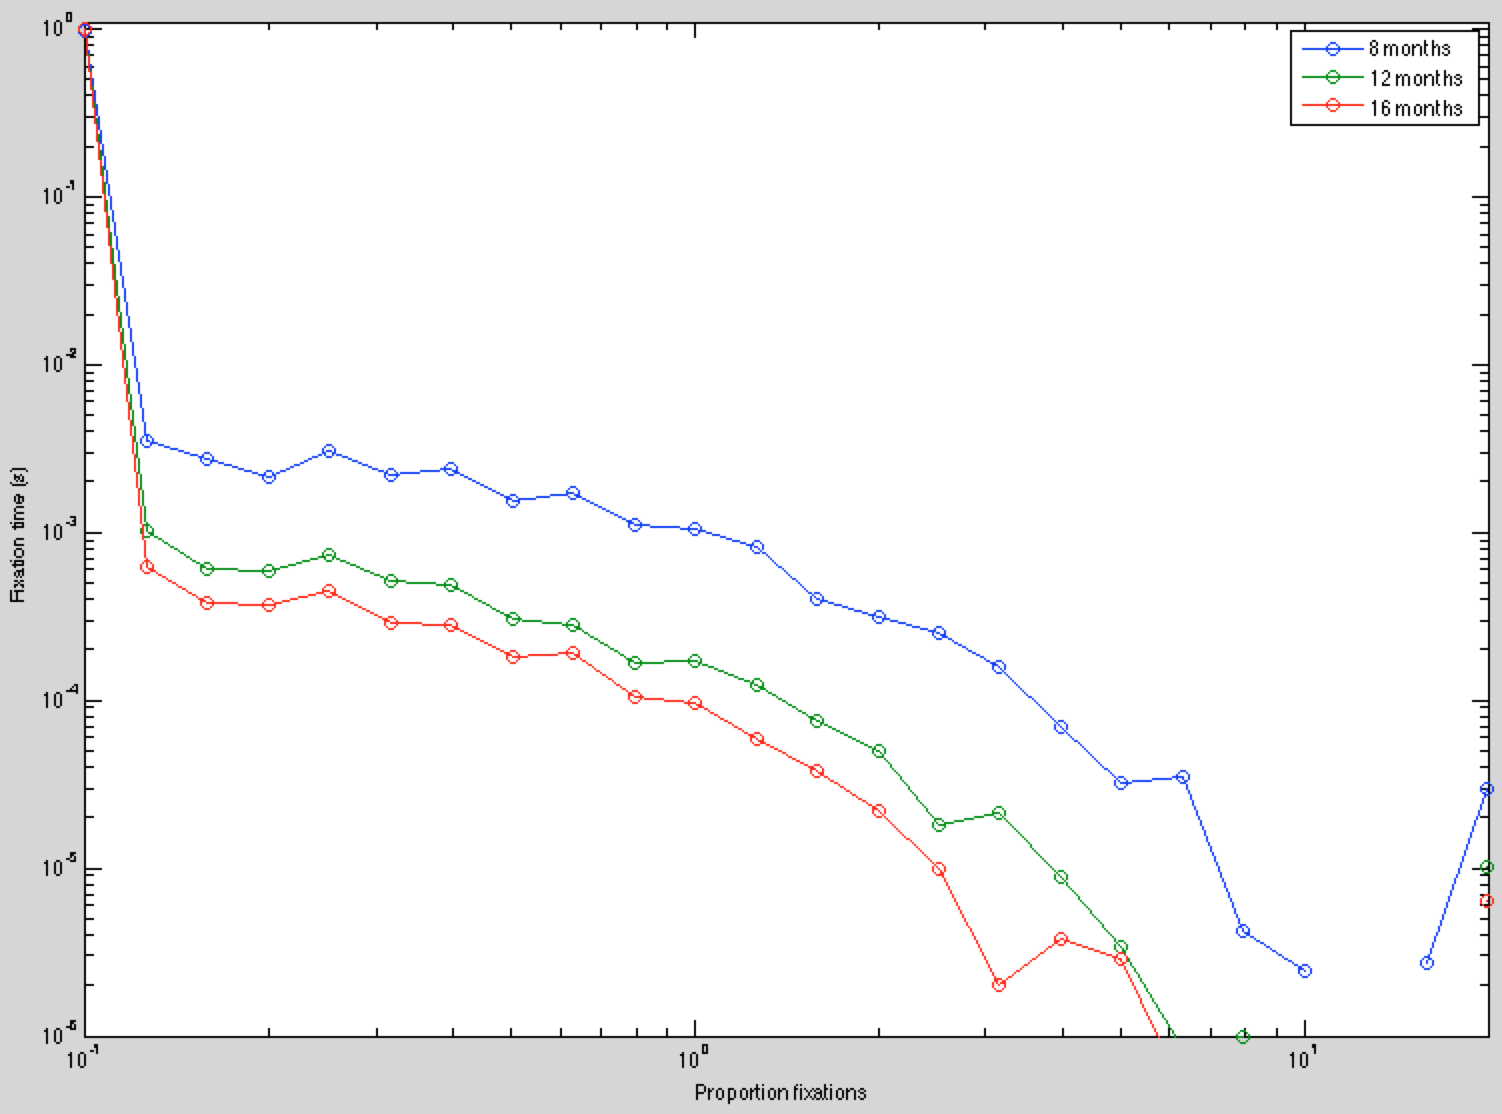
\includegraphics[width=0.45\linewidth]{Image/log2}    \label{fig:buckets}
            }
\caption{Attention Chunks: analyzing the duration in children of 8,12 and 16 month old.}
\label{fig:subfigures}
\end{center}
\end{figure}
\subsection{4. Aggregation: Mapping all features together}
In the previous sections we detected and computed features (faces, objects, etc.) in different cameras. The goal of this stage is to merge and prune the features into a single feature matrix describing the detected features at each video frame.\\

{\bf 4.1. Synchronization.} We calculate the bijective function mapping each frame of the fixed camera to the head mounted camera (i.e. figure \label{fig:main} ). When the inter camera frames can be mapped, the detected features and video attributes of both cameras can also be mapped together.\\

{\bf 4.1. Features definition.} We calculate 6 features for each video $frame_{t}$. 
\begin {itemize}
\item {\bf Chunk Length:} The amount of frames that of the attention chunk containing the $frame_{t}$.
\vspace {-0.2cm}
\item {\bf Chunk Speed:} The average speed of the attention chunk trajectory. 
\vspace {-0.2cm}
\item {\bf Face Speed:} The speed, ($L_{2}$ norm) of the face position at $frame_{t}$ and $frame_{t-1}$.    
\vspace {-0.2cm}
\item {\bf Face Size:} The diagonal of the detected face bounding-box. This feature could characterize the parent-child distance.   
\vspace {-0.2cm}
\item {\bf Object Speed:} The speed, ($L_{2}$ norm) of the handled object position at $frame_{t}$ and $frame_{t-1}$.    
\vspace {-0.2cm}
\item {\bf Object Size:} The diameter of the detected object bounding-ellipse.
\end{itemize}
The lack of detection is replaced by the 0 value. 

{\bf 4.2. Feature shrink an propagation.} The object and face features are computed frame by frame. We use the 

 that are detected in a single video frame occupied by an attention chunk are propagated to all of the frames of the chunk. This step improves the quality of the detection assuming that the attention chunks are strong indicators of the child engaged in a full attention episode.\\ The operation is achieved bu a composition of mapping functions $f ~o~ g$. \\


{\bf 4.3. Normalization.} Dealing with multi-modal features requires of a normalization step. We apply the linear mapping of each feature to the range $[0,1)$ using the minimum and maximum values of each feature vector.\\

\section{Detecting Joint Attention}
Is it possible to automatically detect a complex event such as Joint Attention? Being able to extract analytics of big amounts of data, normally impossible for humans to annotate manually can open new research paths in developmental psychology. We show that the descriptive capabilities of the previously computed features is rich enough to train a joint attention classifier and detect these events in new unseen video frames. We train a naive Bayes Classifier. For each children, the training dataset takes half of the positive and negative Joint Attention feature vectors, and we use the remaining half for testing in a cross validation fashion. 
 
\section{Evaluation}
First order analytics can be extracted of the alignment of the automatic feature detection and the annotations. We map into the video timeline the video segments annotated as JA episode and the face and moving object detection. From the alignment, we compute the percentage of time of the automatic detection occurring inside and outside the manually annotated JA episode. We have performed this for a total 77,825 video frames of 4 different children.  Table 

\begin{table*}
\centering
\begin{tabular}{|c|c|c|c|c|c|c|c|c|c|c|}
\cline{2-6}
\multicolumn{1}{c}{} & \multicolumn{5}{c}{{\bf First order feature analysis}} 
\\
\cline{2-6}
\multicolumn{1}{c|}{} &\%Faces IN & \%Faces OUT & \%Toy IN & \% Toy OUT & Total frames\\
\hline\\[-1.2em]\hline
Child 0807 &  19\%        & 4\%    &  85\%  &  $<$ 0\%& 19284\\
\hline\
Child 0815 &   21\%       & 5\%    &  51\%   &$<$ 0\%& 22421\\
\hline\
Child 1604 &   29\%       & 16\%  &  44\%   & $<$ 0\%  & 19337\\
\hline\
Child 0801 &   8\%         &  4\%   &  11\%   & 11\%  & 16783\\
\hline
Child 1612 &   8\%         &  4\%   &  11\%   & 11\%  & 13450\\
\hline
\end{tabular}
\caption{The table shows the percentage (normalized by time) of detected faces and handled object inside and outside a JA episode. The distribution of faces and handled object is dense inside the JA episode showing that those features are indicators of a JA episode.}
\label{tb:Results2}
\end{table*}
\begin{figure}[h]
     \begin{center}
          \subfigure[Weight distribution of the features learned by the model. Each graph represents and an independent experiment, still the inter experiments weight relationship is similar.]{%
           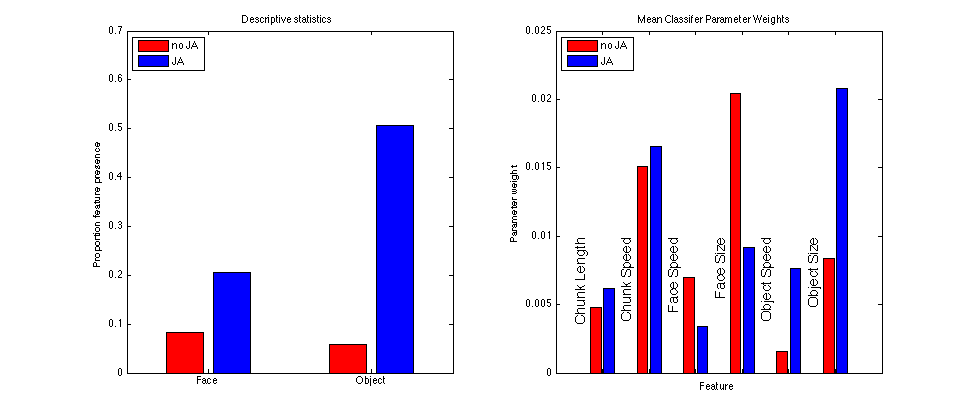
\includegraphics[width=1\linewidth]{Image/weights} 
           }
        \subfigure[Average weights inter models. The results show that the most discriminative feature ha a strong relationship with the handled object, followed by the detection of faces.]{%
           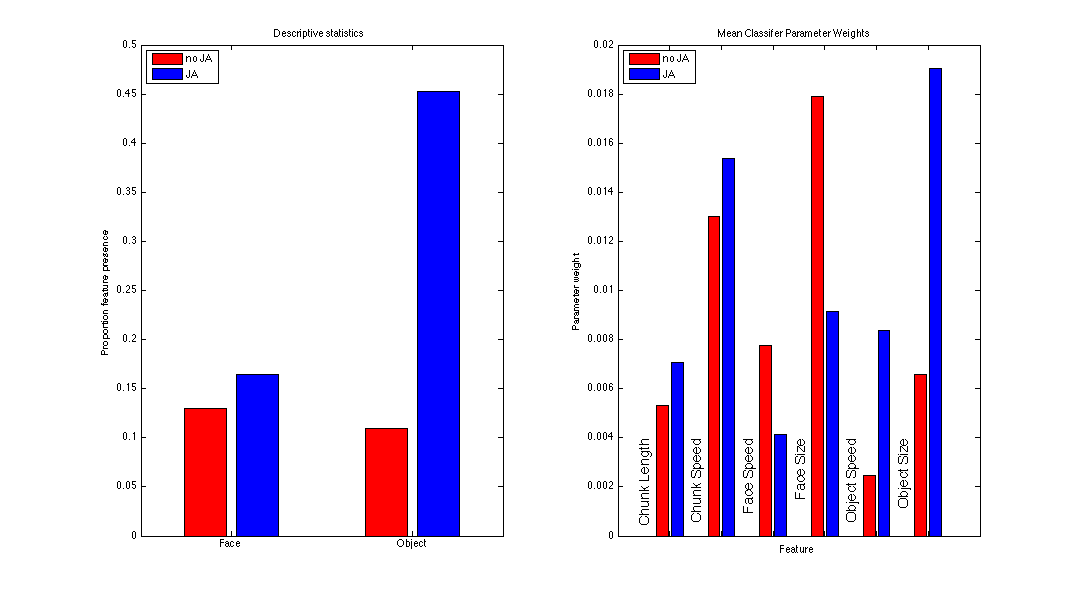
\includegraphics[width=1\linewidth]{Image/individual} 
           }
          \end{center}
    \caption{todo... 
     }
   \label{fig:main}
\end{figure}
{\bf The benefits of the attention chunk:} We evaluate the same approach removing the attention chunk shrinking and propagation step. The accuracy of the classifier dropped down an average of 7\% in accuracy. 
\subsection{Results}

\section{Conclusions}
This paper aims at better understanding the episodes of joint attention by computing a set of features (i.e. Attention Chunks, Face, Object handling) which can drive to the automatic detection of Joint Attention. In this paper, 3 conclusions emerge. First, the motion of an object that is being part of a child-parent interaction are an important cue for joint attention detection. Second, the detection of sustained attention is a good proxy to improve the detection of joint attention. 
Third, the motion of objects is important when the children are playing interactively with the parents, but then children have locomotion capabilities the object motion is not a strong cue of joint attention.
\bibliographystyle{apacite}

\setlength{\bibleftmargin}{.125in}
\setlength{\bibindent}{-\bibleftmargin}

\bibliography{ja}

\section{Appendix: Joint Attention presence annotation}
Joint attention was defined if it satisfied the criteria by Tomasello and Todd (1983). First, the interaction had to begin with either the parent or child initiating the interaction. For example, a parent could hold up an object and label it, or a child could bring an object over the parent. Second, both members focus on the single object for at least 3 seconds (including brief glances away). Third, at some point during the interaction the child must display an overt behavior towards the parent to show that he is aware of the interaction. 
\end{document}
